\documentclass[10pt,a4paper]{labreport}
\usepackage{csquotes}
\usepackage{titlesec}
\usepackage{ragged2e}
\usepackage{siunitx}
\usepackage{setspace}
\usepackage{longtable}
\usepackage{rotating}
\usepackage{xurl}
\usepackage{physics}
\usepackage{caption}
\usepackage{wrapfig}
\usepackage{tabularray}
\usepackage{fancyhdr}
\usepackage{subcaption}
\usepackage{lscape}
\usepackage{tensor}
\usepackage{multirow}
\usepackage{chemformula}
\usepackage[gen]{eurosym}
\usepackage{float}
\usepackage{bm}
\usepackage{lipsum}
\usepackage{parskip}
\usepackage{booktabs}
\usepackage{amsmath}
\usepackage{enumerate}
\usepackage[justification=justified]{caption}
\usepackage[nottoc]{tocbibind}
\usepackage{hyperref}
\usepackage[
backend=biber,
style=chem-acs,articletitle=true,doi=true]{biblatex}
\addbibresource{references.bib}
\usepackage{color}

\usepackage{listings}
\definecolor{codegreen}{rgb}{0,0.6,0}
\definecolor{codegray}{rgb}{0.5,0.5,0.5}
\definecolor{codepurple}{rgb}{0.58,0,0.82}
\definecolor{backcolour}{rgb}{0.95,0.95,0.92}
\lstdefinestyle{mystyle}{
    backgroundcolor=\color{backcolour},   
    commentstyle=\color{codegreen},
    keywordstyle=\color{codepurple},
    numberstyle=\tiny\color{codegray},
   % stringstyle=\color{grey},
    basicstyle=\ttfamily\footnotesize,
    breakatwhitespace=false,         
    breaklines=true,                 
    captionpos=b,                    
    keepspaces=true,                 
    numbers=left,                    
    numbersep=5pt,                  
    showspaces=false,                
    showstringspaces=false,
    showtabs=false,                  
    tabsize=5
}
\lstset{style=mystyle}





\title{Nanoscale Material Modelling
\\
\normalsize{Week 2}} % Main title and sub title. 

\author{Ilija A. Gjerapić, S4437586; \href{mailto:i.a.gjerapic@student.rug.nl}{i.a.gjerapic@student.rug.nl}; \href{https://github.com/igjerapic/nmm-week2/}{@github} } % Name, student number, email

\supervisors{prof. dr. A. Giuntoli, prof. dr. J. Slawinska}

\begin{document}


\maketitle

\tableofcontents


  

\thispagestyle{firststyle}
\newpage
\section{Assignment 1: DFT calculation of Bulk Si}
The input files were modified to include lattice constants of \{9.8, 10.0, 10.26, 10.4, 10.6\} Bohrs by modifying the  \texttt{celldm(1)} in the \texttt{system} namelist of the \texttt{quantum expreso} input file. The \texttt{ibrav} variable was set to 2, corresponding to a FCC structure, thus this change in lattice structure corresponds to the side of the FCC lattice. 

The total energies of each lattice constant was extracted using the \texttt{bash} script shown in listing \ref{lst:ass1_totEng} and are shown in Figure \ref{fig:ass1}. 
The optimized lattice constant, with the minimal total energy was determined to be 5.50 \AA. 
This result is larger than the reported literature value of 5.43 {\AA} \cite{homAccurateLatticeConstants1975}. 

\begin{lstlisting}[language=bash, 
    caption={The shell script used to extract and store the total energies from the finished simulations of different lattice constants.},
    label=lst:ass1_totEng,
    ]
#!/bin/bash

rm etot-v-lat_const
for lat_const in 9.8 10.0 10.26  10.4 10.6; do
    dir_name="Si_${lat_const}"
    outfile="$dir_name/Si.scf.out"
    
    etot=$(grep -e ! $outfile | awk '{print $(NF-1)}')
    
    echo "$lat_const    $etot" >> etot-v-lat_const
done
\end{lstlisting}

\begin{figure}[h]
    \centering 
    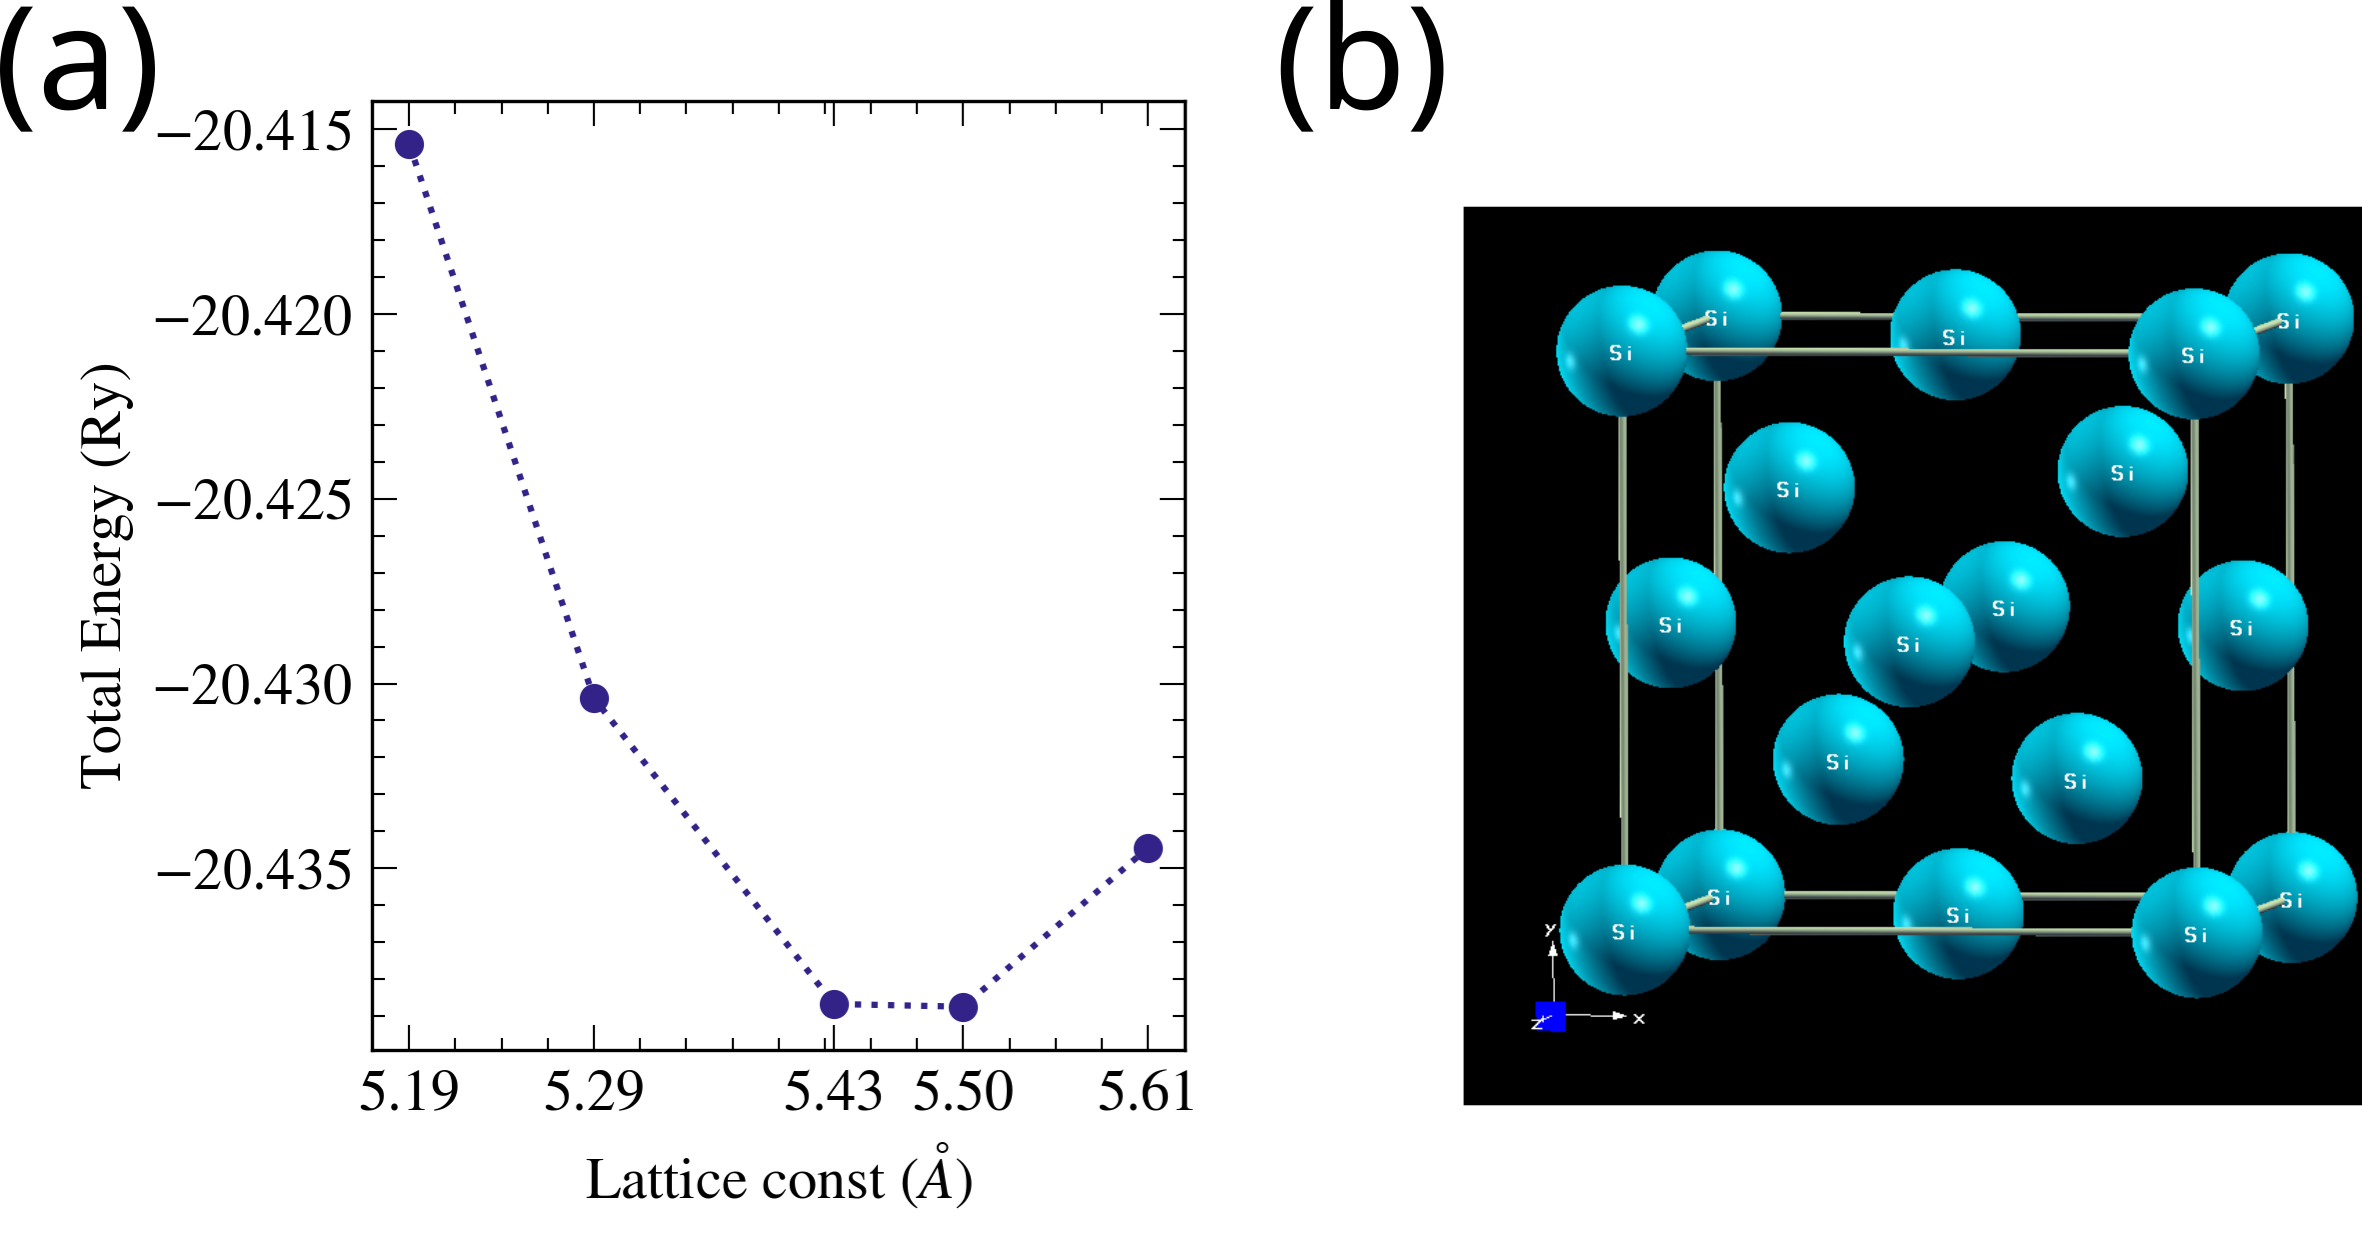
\includegraphics[width = 0.7 \textwidth]{figs/ass1.png}
    \caption{ (a) The total energy plotted against the lattice constant of the bulk Si FCC structure. The optimized lattice constant was determined to be 5.50 \AA. (b) The structure of bulk silicon corresponding to the optimal lattice structure. }
    \label{fig:ass1}
\end{figure}

\newpage
\section{Assignment 2: DOS of Bulk Si}
The density of states was calculated for the optimal crystal lattice constant calculated is shown in Figure \ref{fig:ass2}. The density of states provides an energy gap of 0.77 eV between the highest occupied state and the lowest unoccupied state, which corresponds to an insulator. 

\begin{figure}[h]
    \centering 
    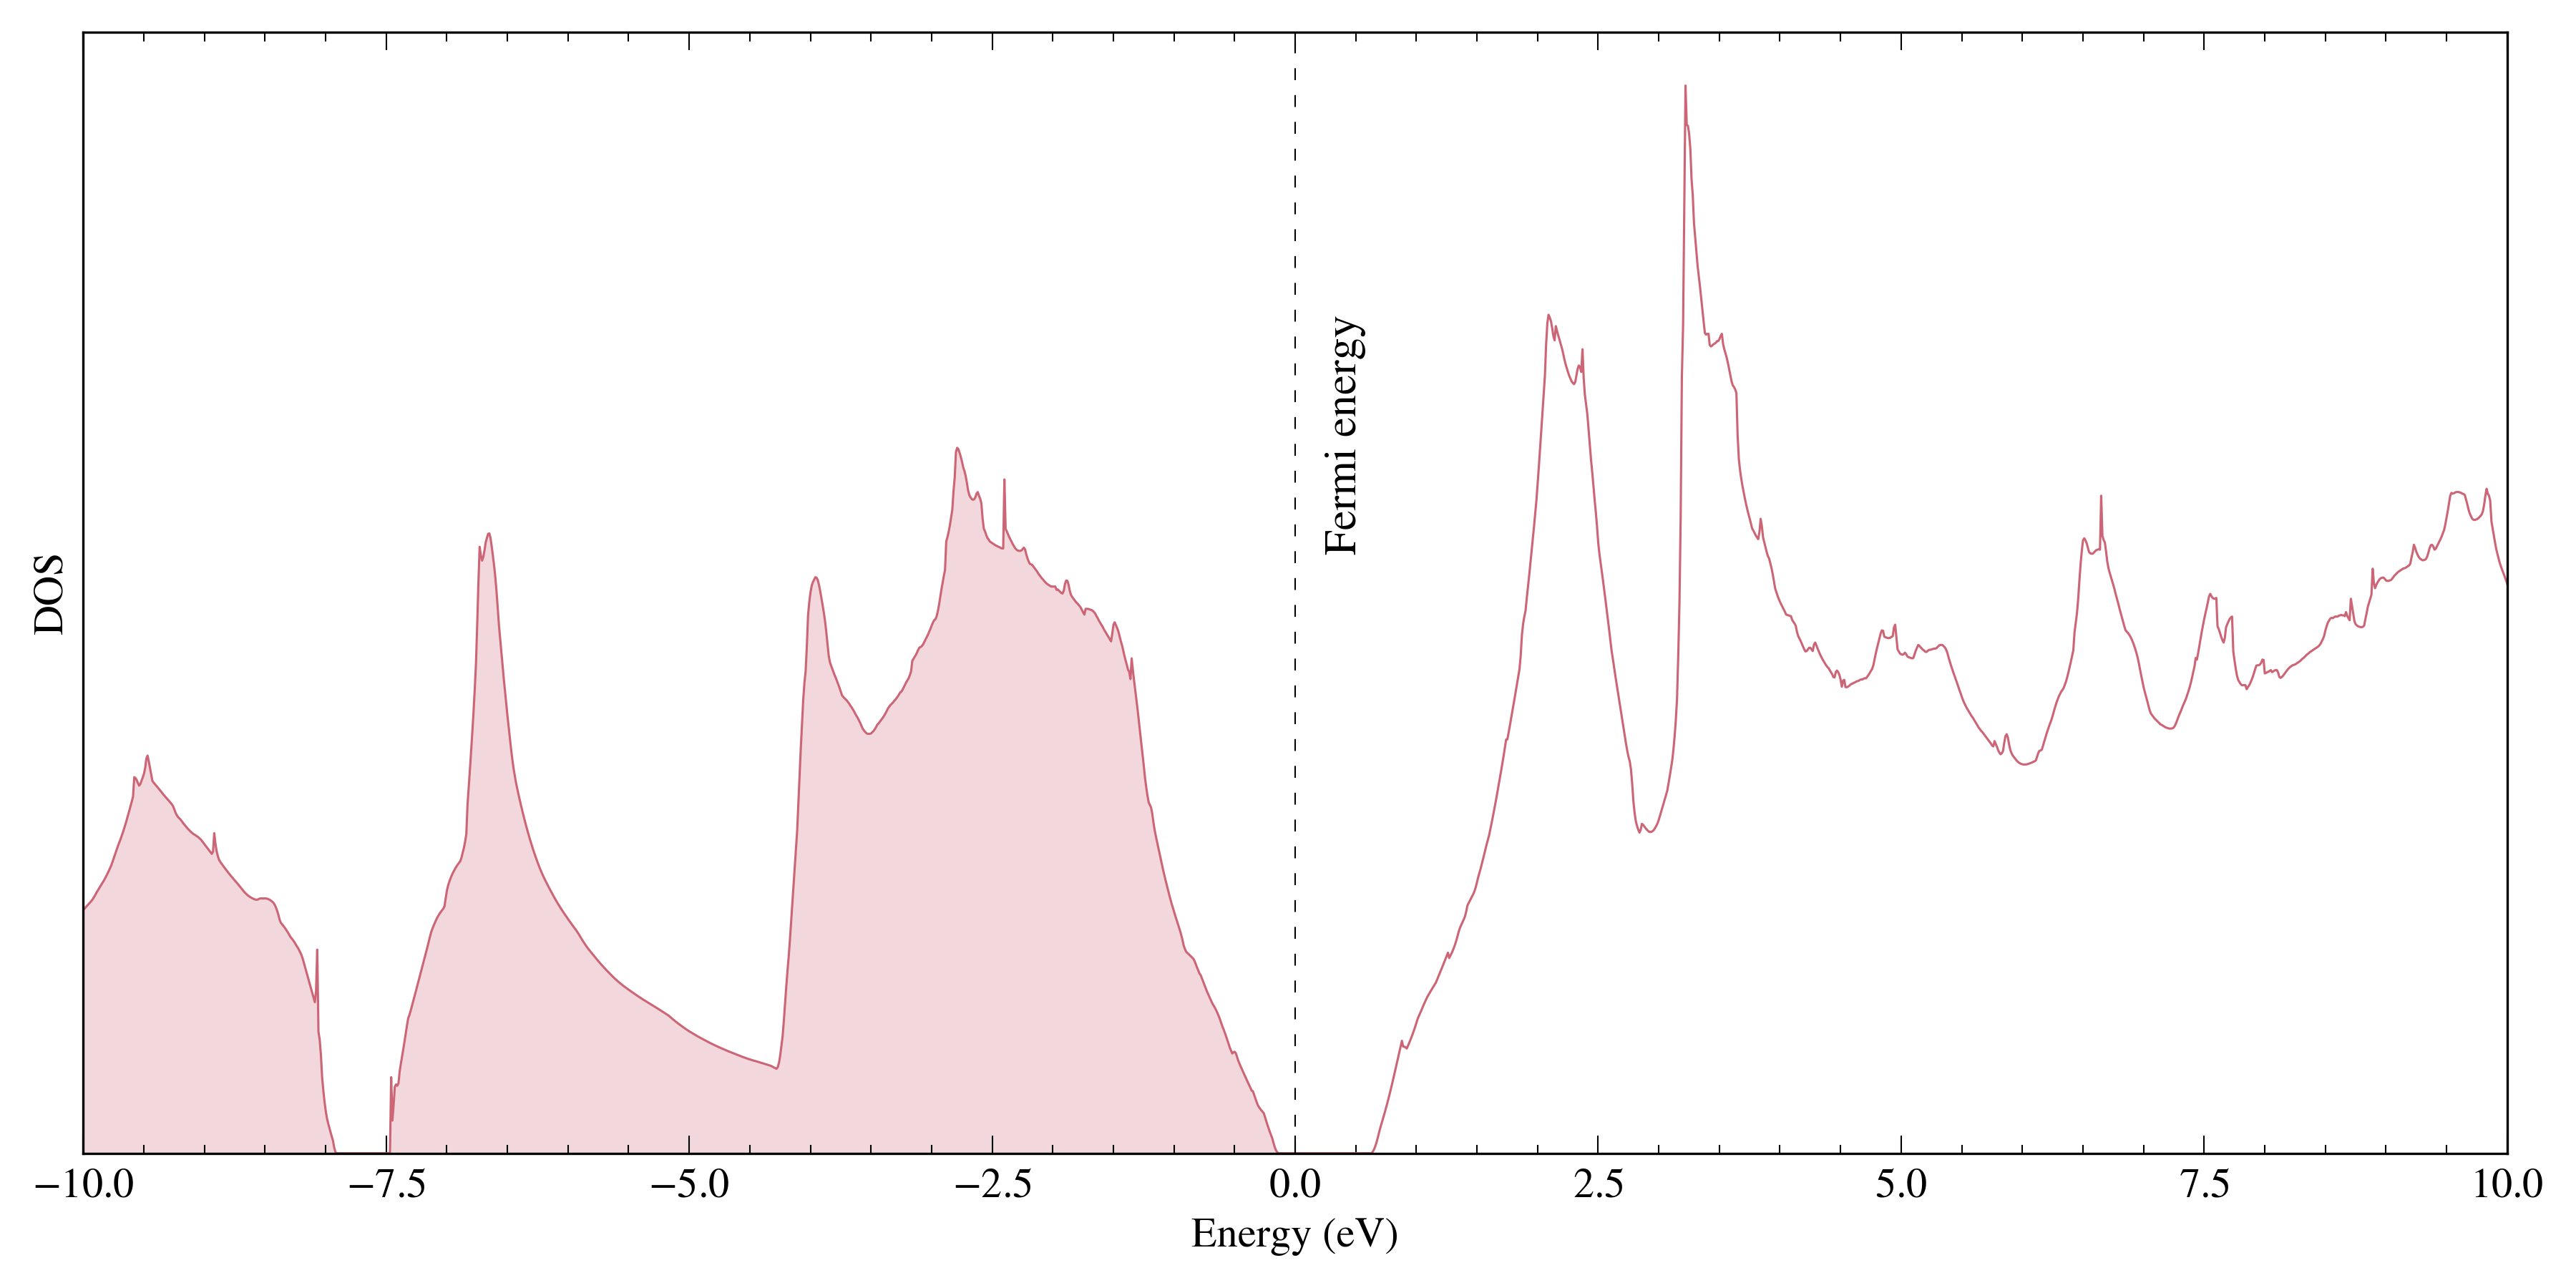
\includegraphics[width = 0.7 \textwidth]{figs/ass2_dos.png}
    \caption{The density of states of bulk Silicon with a lattice constant of 5.50 \AA. There is an energy gap of 0.77 eV, between the highest occupied state and the lowest unoccupied state making bulk silicon a semiconductor.}
    \label{fig:ass2}
\end{figure}

\newpage
\section{Assignment 3: Electronic Structure Bulk Si}
The high-symmetry point path chosen to outline the electronic structure of bulk silicon is shown in Figure \ref{fig:ass3_kpoints}. 

\begin{figure}[h]
    \centering 
    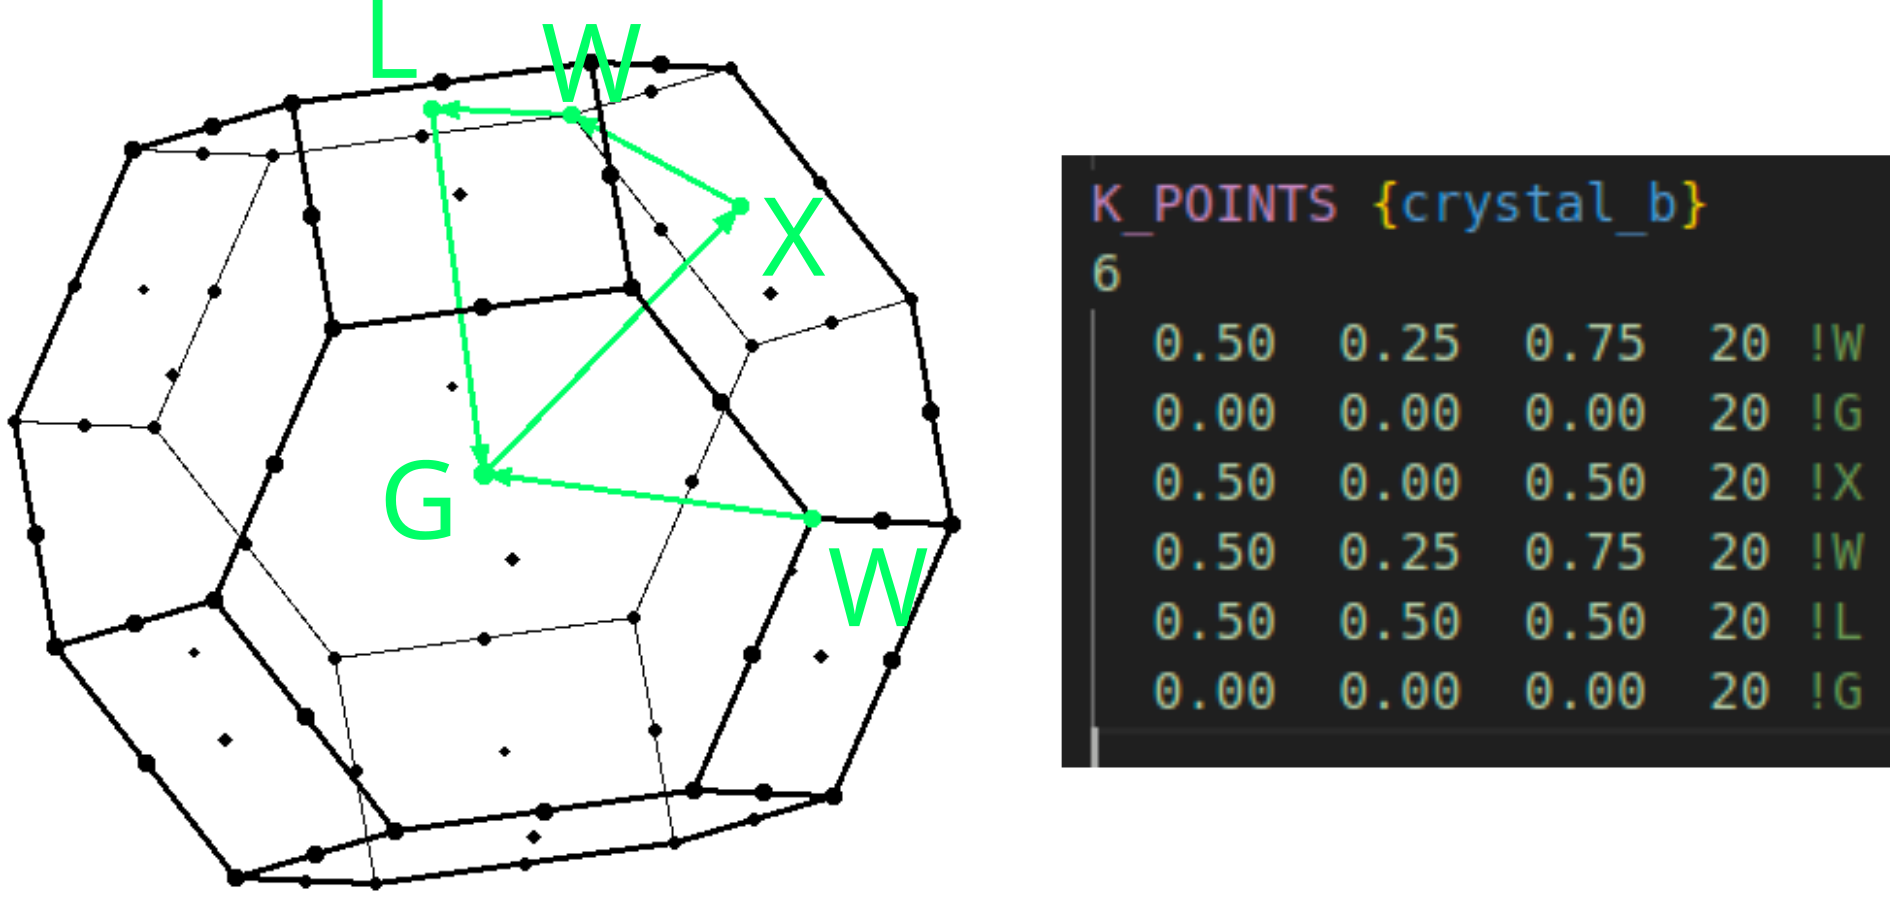
\includegraphics[width = 0.7 \textwidth]{figs/ass3_kpoints.png}
    \caption{The path along the high-symmetry points (left) and their coordinates with respect to the vectors of the Brillouin zone (right) used to calculate the electronic structure of bulk silicon.}
    \label{fig:ass3_kpoints}
\end{figure}

Figure \ref{fig:ass3_bands} shows the resulting electronic structure. This differs from literature mainly in the path sections of W-G and W-L in that there are two bands with energy greater than -4 eV rather than one. This is likely due to the larger lattice structure determined from the calculations.  

\begin{figure}[h]
    \centering 
    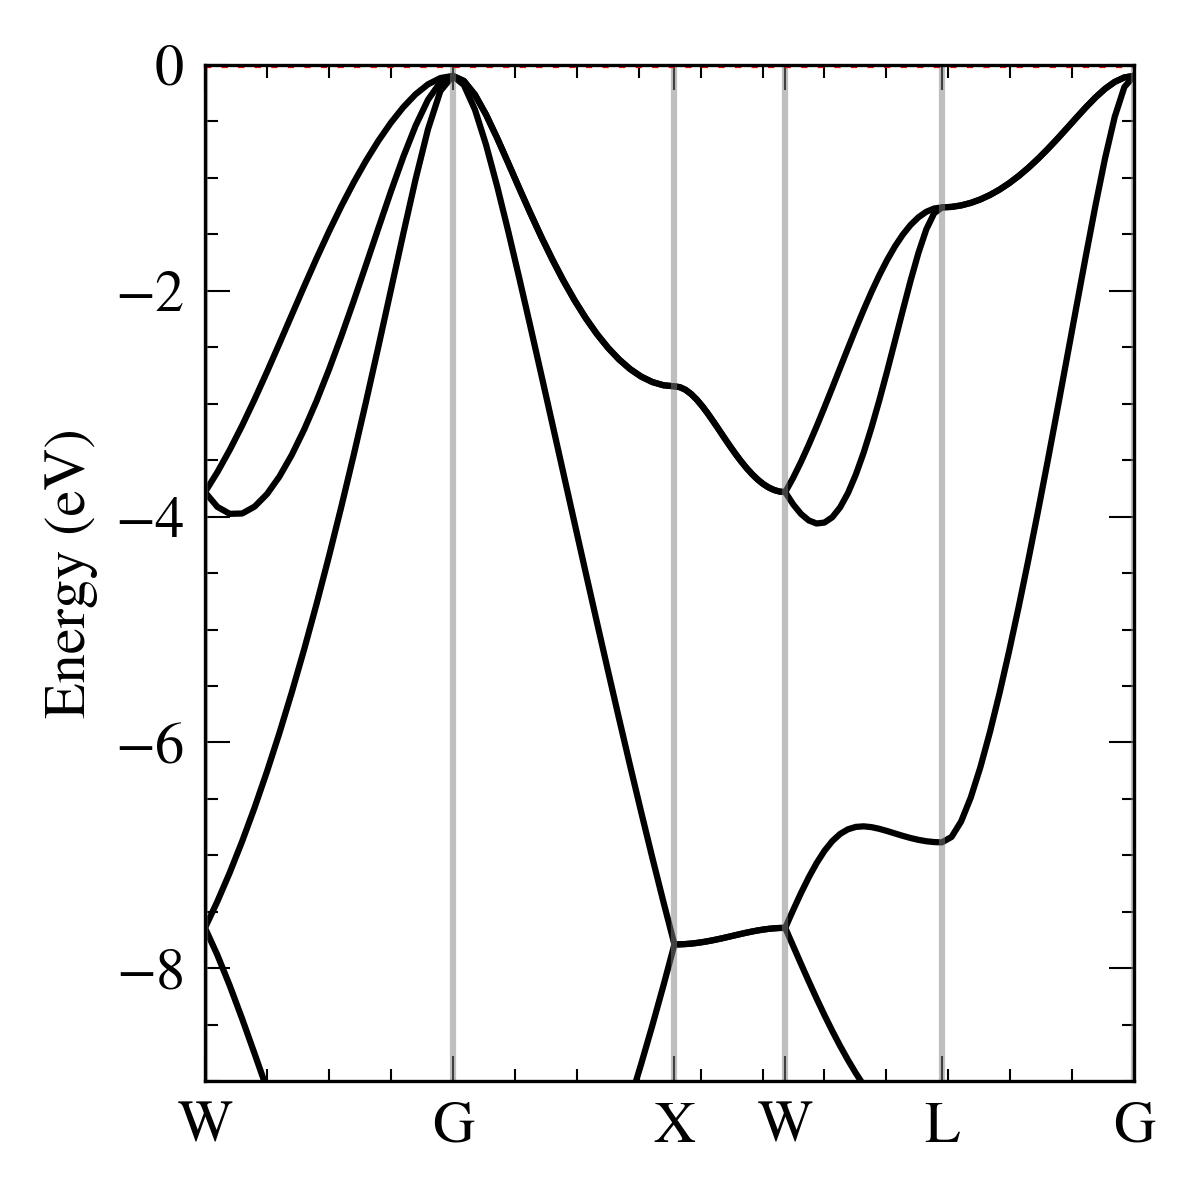
\includegraphics[width = 0.5\textwidth]{figs/ass3_bands.png}
    \caption{The resulting band structure from a bulk silicon structure with lattice constant of 5.50 \AA. }
    \label{fig:ass3_bands}
\end{figure}


\newpage
\section{Assignment 3: Graphite}

\subsection{Structure Optimization}
To provide the structure of graphite, the \texttt{system} section of the input file was changed to correspond with a hexagonal lattice as shown in listing \ref{lst:ass4_graphiteSyst}.  As graphite is a Van der Waal material, the semi-emperical Grimme's DFT-D3 correction was used during the structure optimization. 

\begin{lstlisting}[language=Perl, 
    caption={The change to the \texttt{system} section of the input file. celldm(1) corresponds to the lattice paramters 'a', while celldm(3) is the ratio between lattice constants: c/a.},
    label=lst:ass4_graphiteSyst,
    ]
&system    
  ibrav=  4, 
  celldm(1)= 4.641, 
  celldm(3)= 2.726, 
  nat=  4, 
  ntyp= 1,
  ecutwfc= 40.0
  vdw_corr= 'DFT-D3'
\end{lstlisting} 

% To optimize the structure, both the lattice constant $a$ and ratio between lattice constant $c/a$ were varied with $\a \in \{4.441, 4.541, 4.641, 4.741, 4.841\}$ Bohr $c/a \in \{ 2.526,  2.626, 2.726, 2.826, 2.926 \}$. 

Figure \ref{fig:ass4_structopt} shows the results of the structure optimization. The optimized structure has lattice dimensions of $a$ = 4.641 Bohr = 2.456 {\AA} and $c/a = 2.726$. This is great agreement with literature values of $a=2.46${\AA} and $c/a = 2.723$ \cite{hembacherRevealingHiddenAtom2003}. 

\begin{figure}[h]
    \centering 
    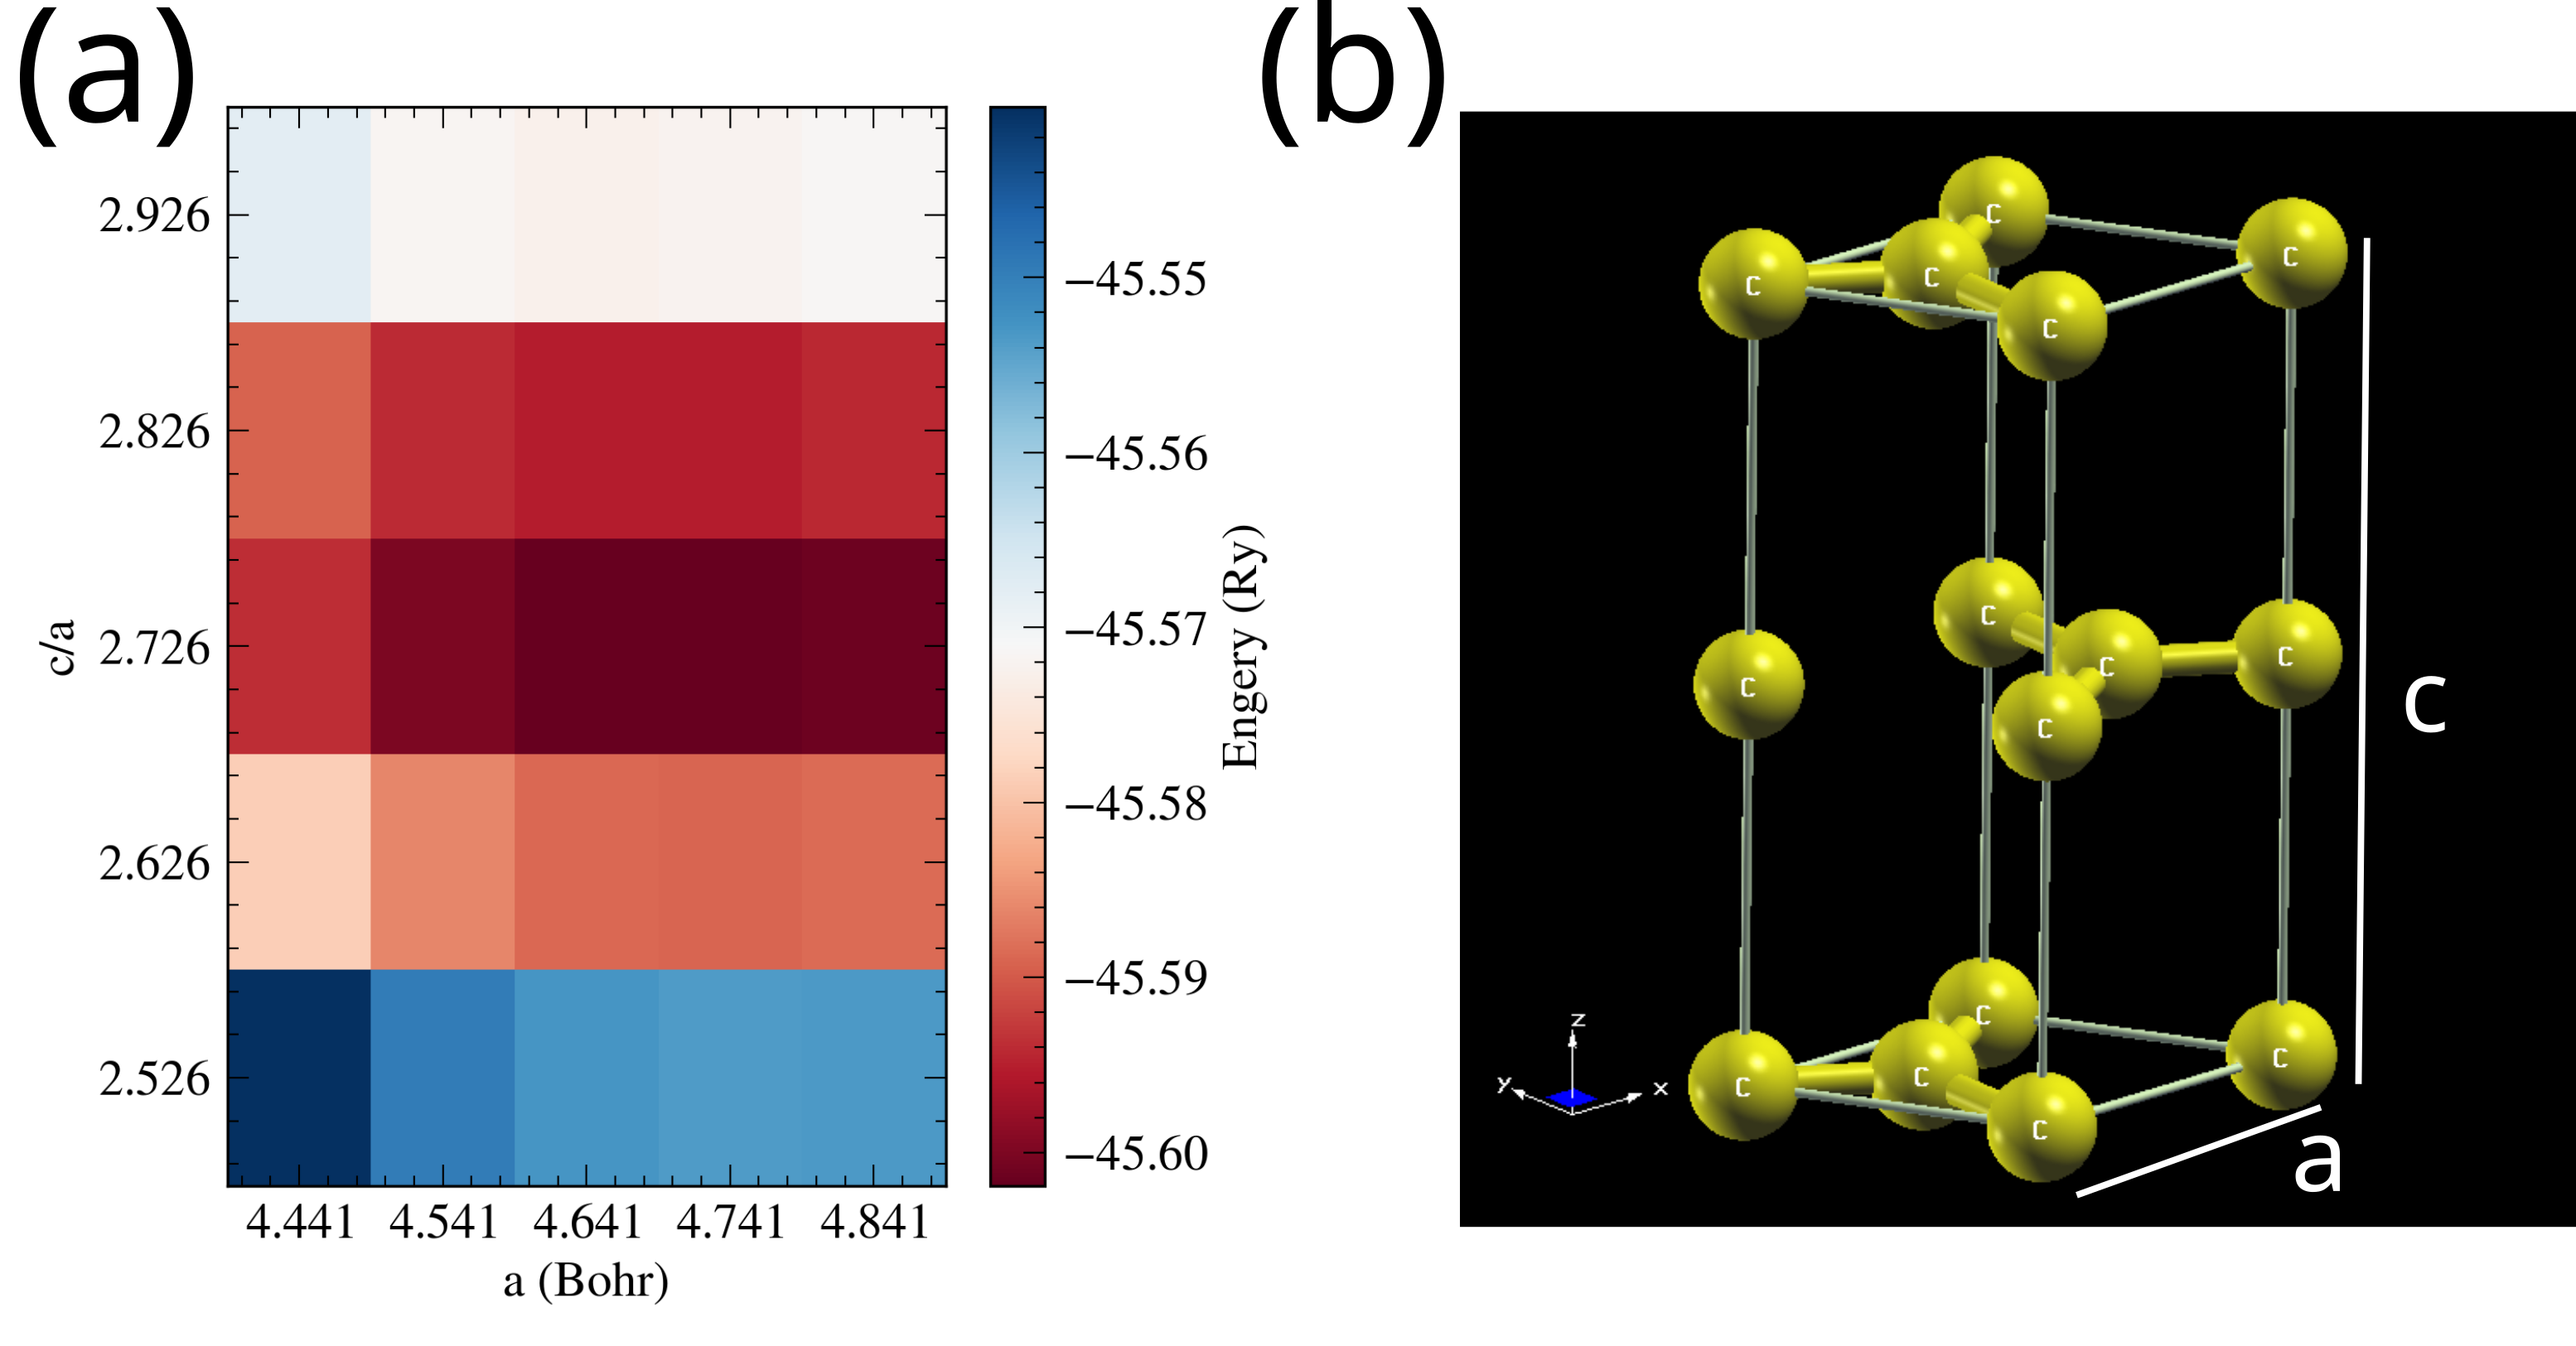
\includegraphics[width = 0.75\textwidth]{figs/ass4_structopt.png}
    \caption{ (a) The total energy plotted as a heat map with respect to the different lattice parameters of the Graphite structure. The
            optimal lattice parameters were determined to be $a = 4.641$ Bohr $=2.456${\AA} and $c/a = 2.726$. (b) An example of a simulated graphite structure with the lattice parameters labeled. }
    \label{fig:ass4_structopt}
\end{figure}

\newpage
\subsection{Density of States}
The density of states for $a=2.456${\AA} and $c/a = 2.726$ is shown in Figure \ref{fig:ass4_dos}. There are some occupied energy states above the Fermi energy, thus graphite is a conductor. 

\begin{figure}[h]
    \centering 
    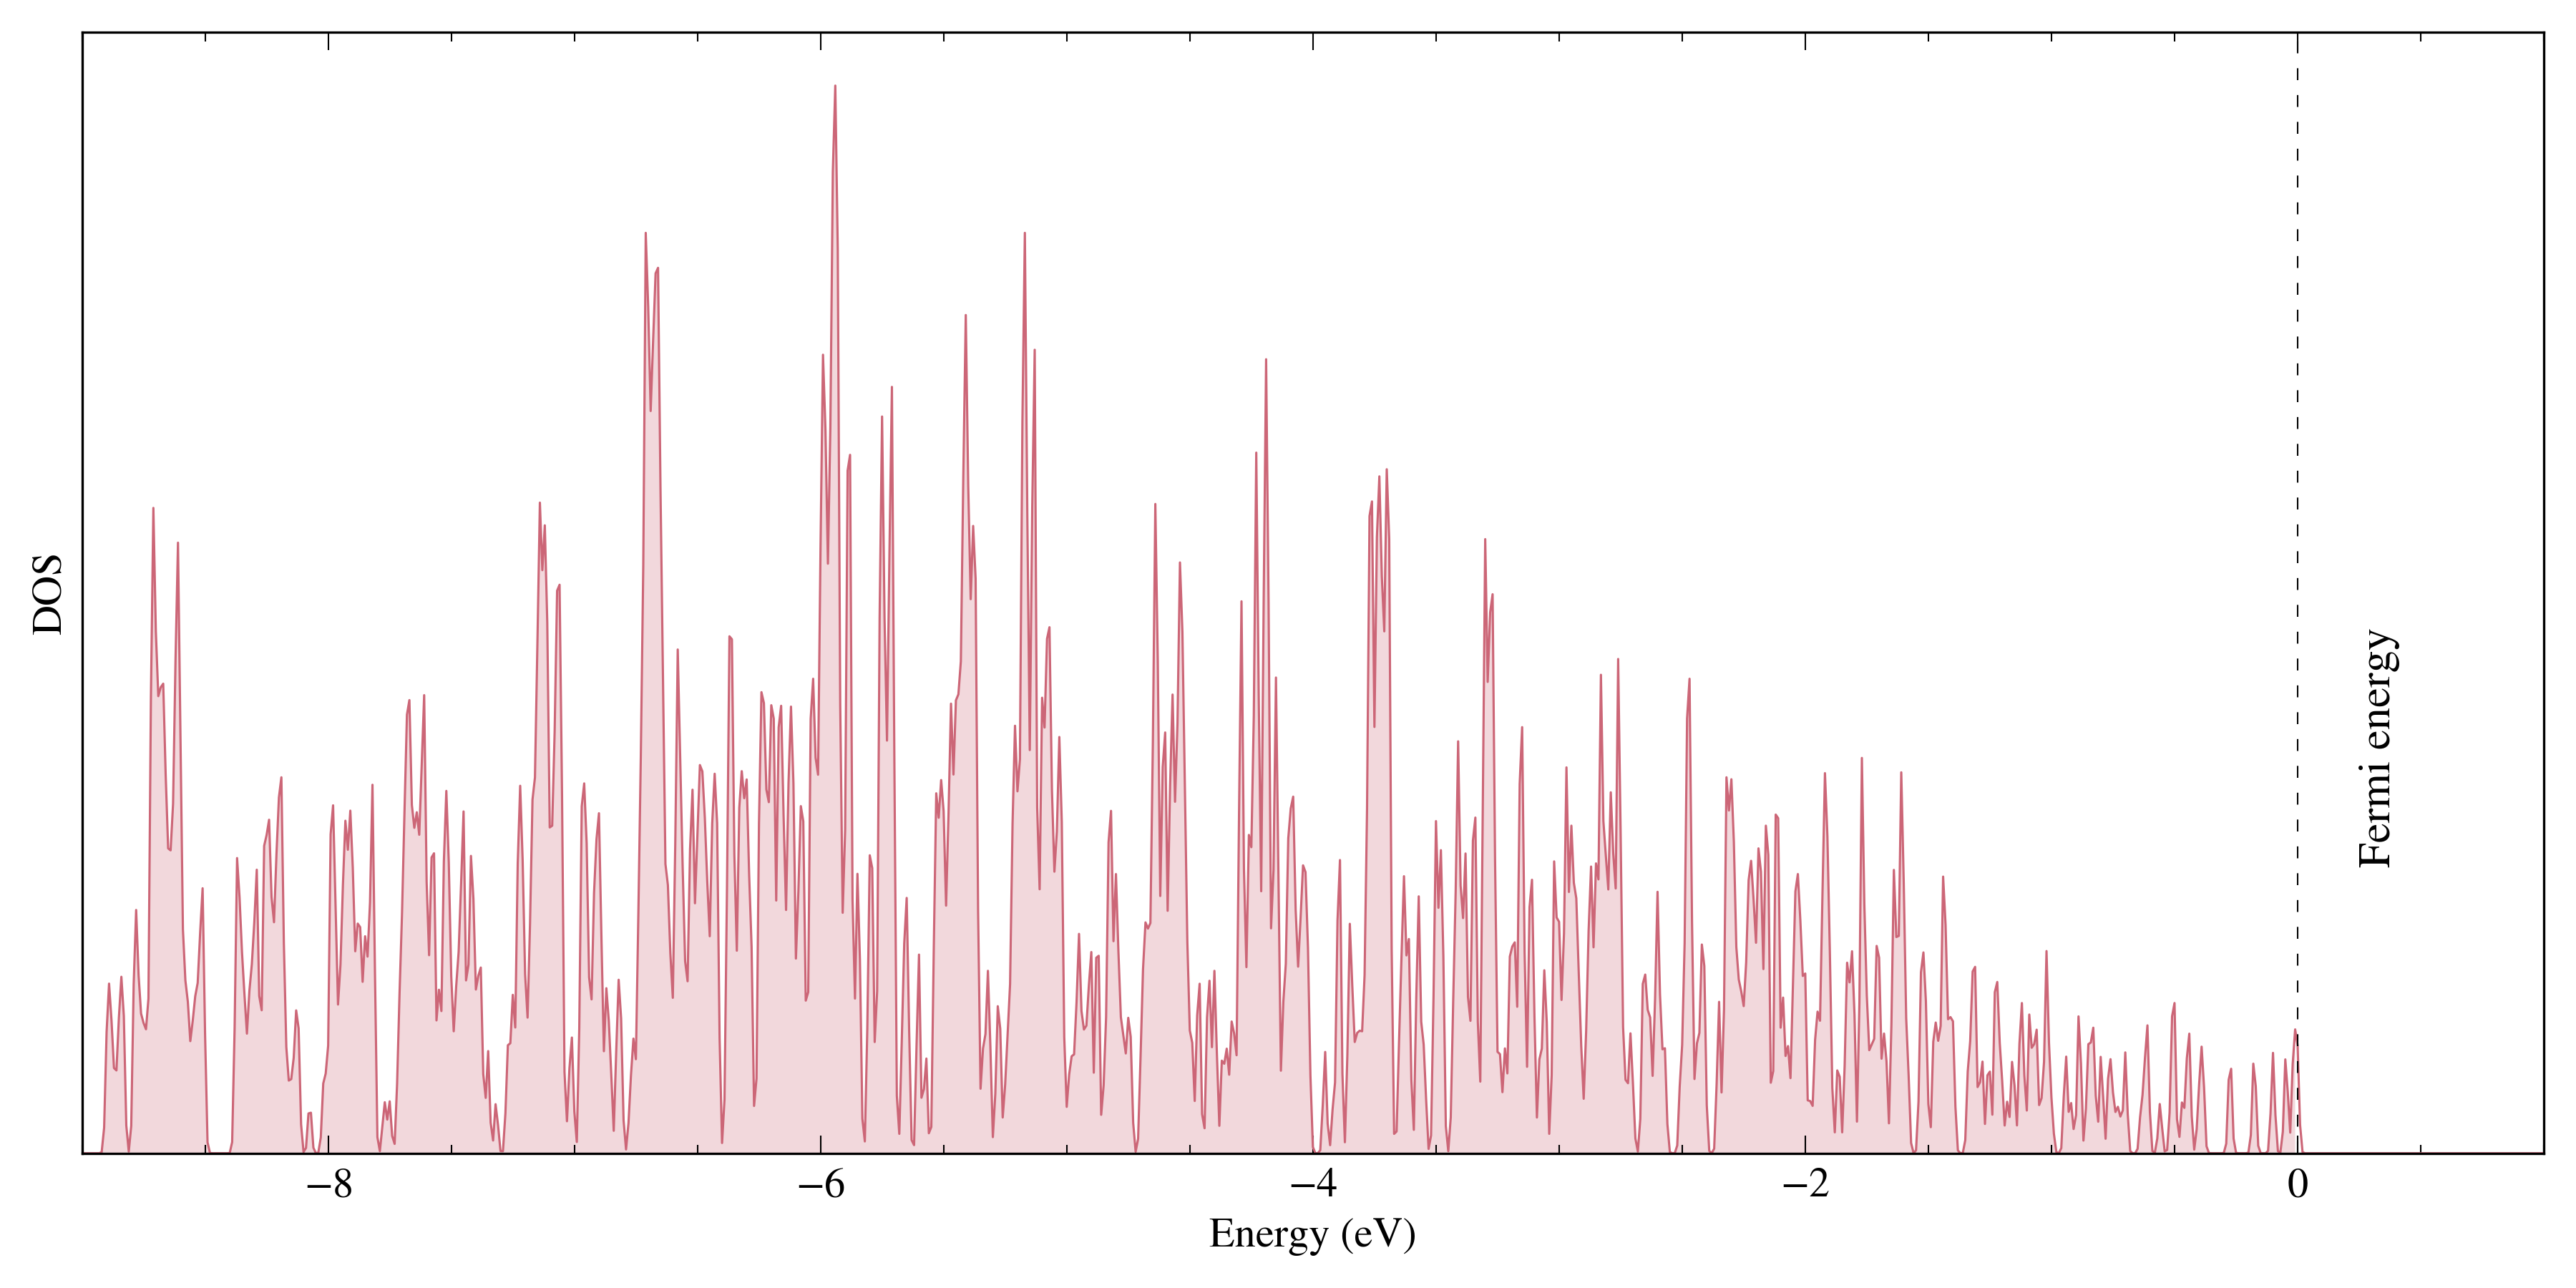
\includegraphics[width = 0.7\textwidth]{figs/ass4_dos.png}
    \caption{ The density of states of bulk graphite with the optimized lattice parameters. Only occupied energy states are shown. As there exist occupied energy states above the Fermi energy, graphite is a conductor. }
    \label{fig:ass4_dos}
\end{figure}

\subsection{Band Diagram}
The band structure of Graphite was calculated along the path M-G-K-M as shown in Figure 

\begin{figure}[h]
    \centering 
    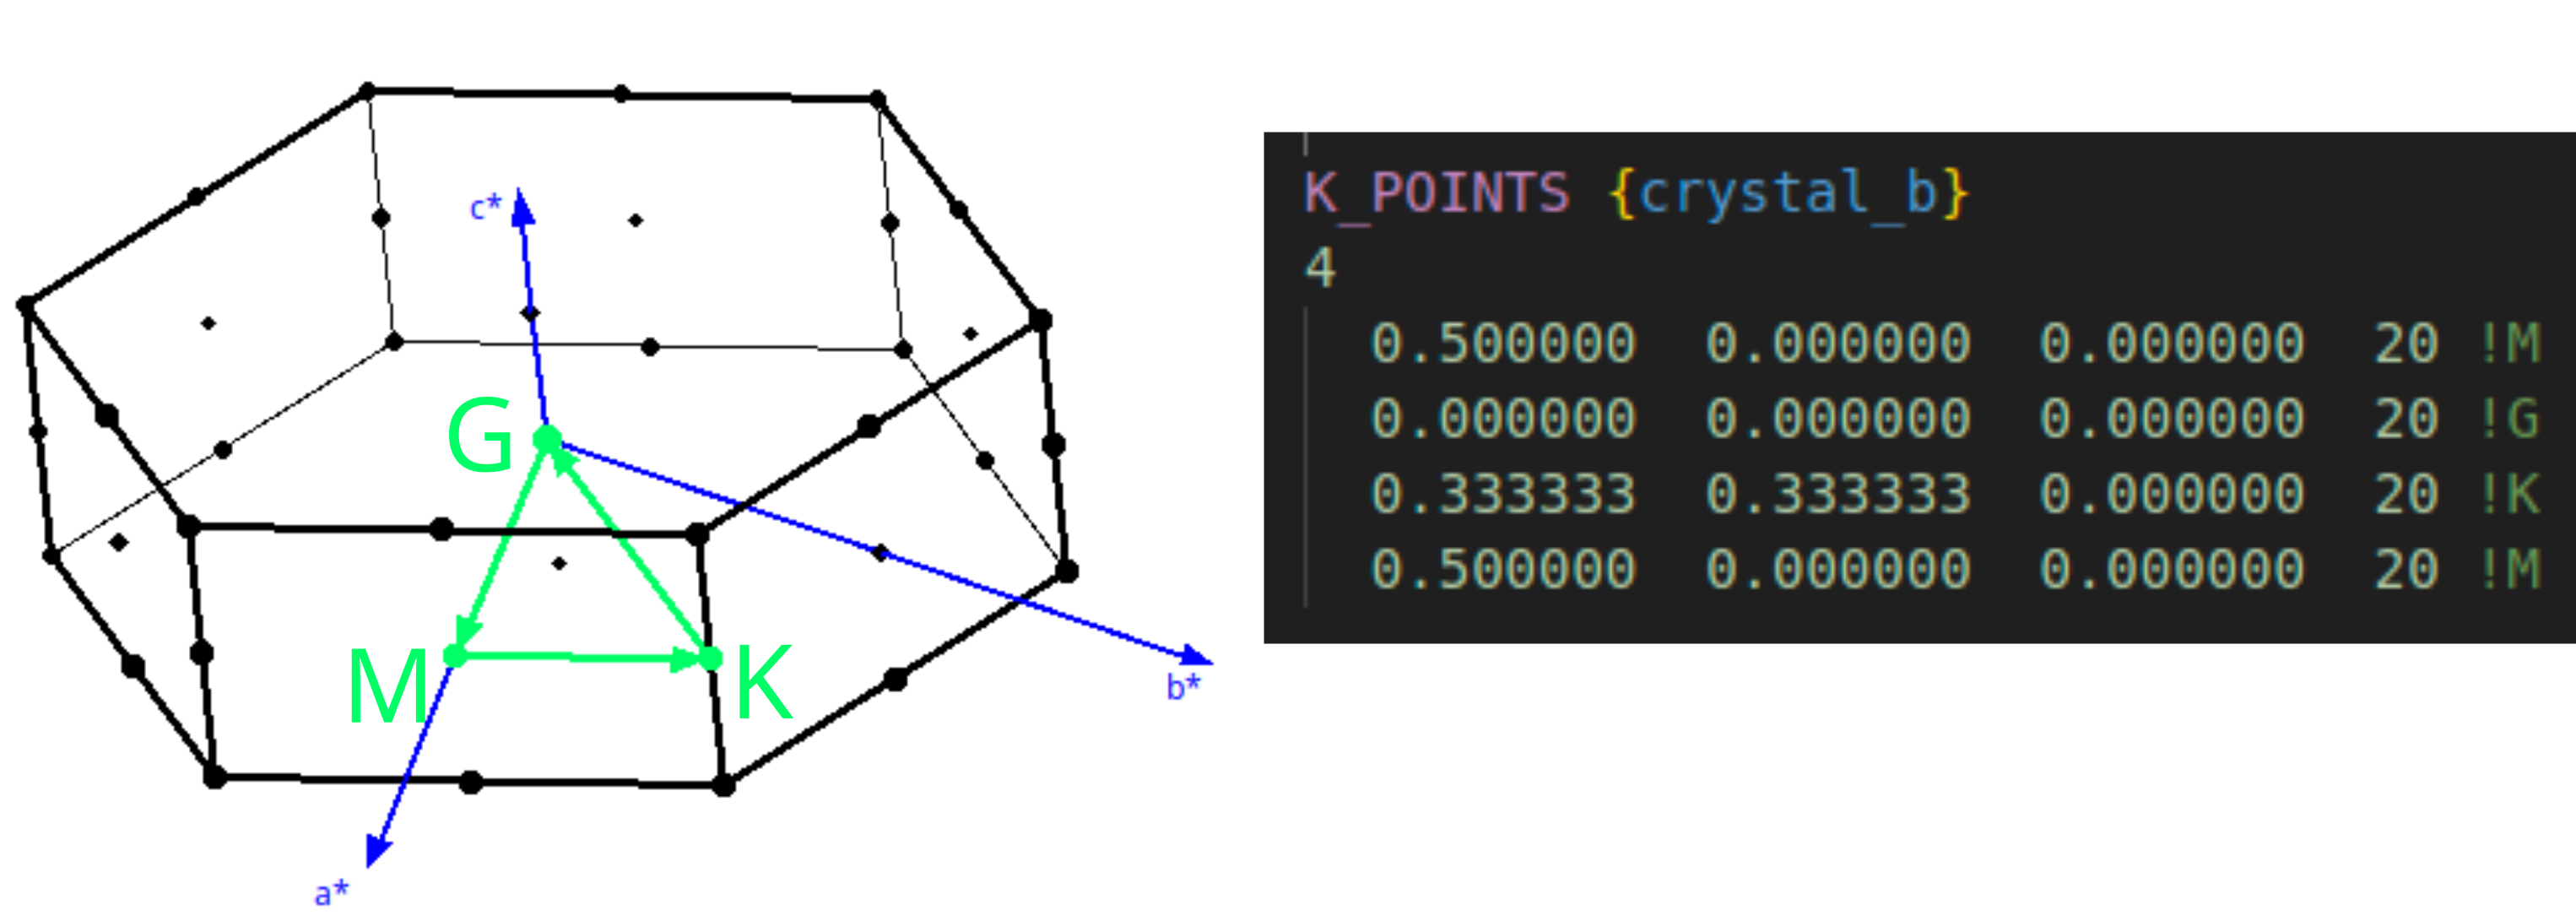
\includegraphics[width = 0.7\textwidth]{figs/ass4_kpoints.png}
    \caption{ The path along the high-symmetry points (left) and their coordinates with respect to the vectors of the Brillouin zone (right) used to calculate the electronic structure of bulk graphite.}
    \label{fig:ass4_kpoints}
\end{figure}

Figure \ref{fig:ass4_bands} shows the resulting band structure with comparison to literature \cite{newsonDynamicsCarriersPhotoinjected2010a}. 

\begin{figure}[h]
    \centering 
    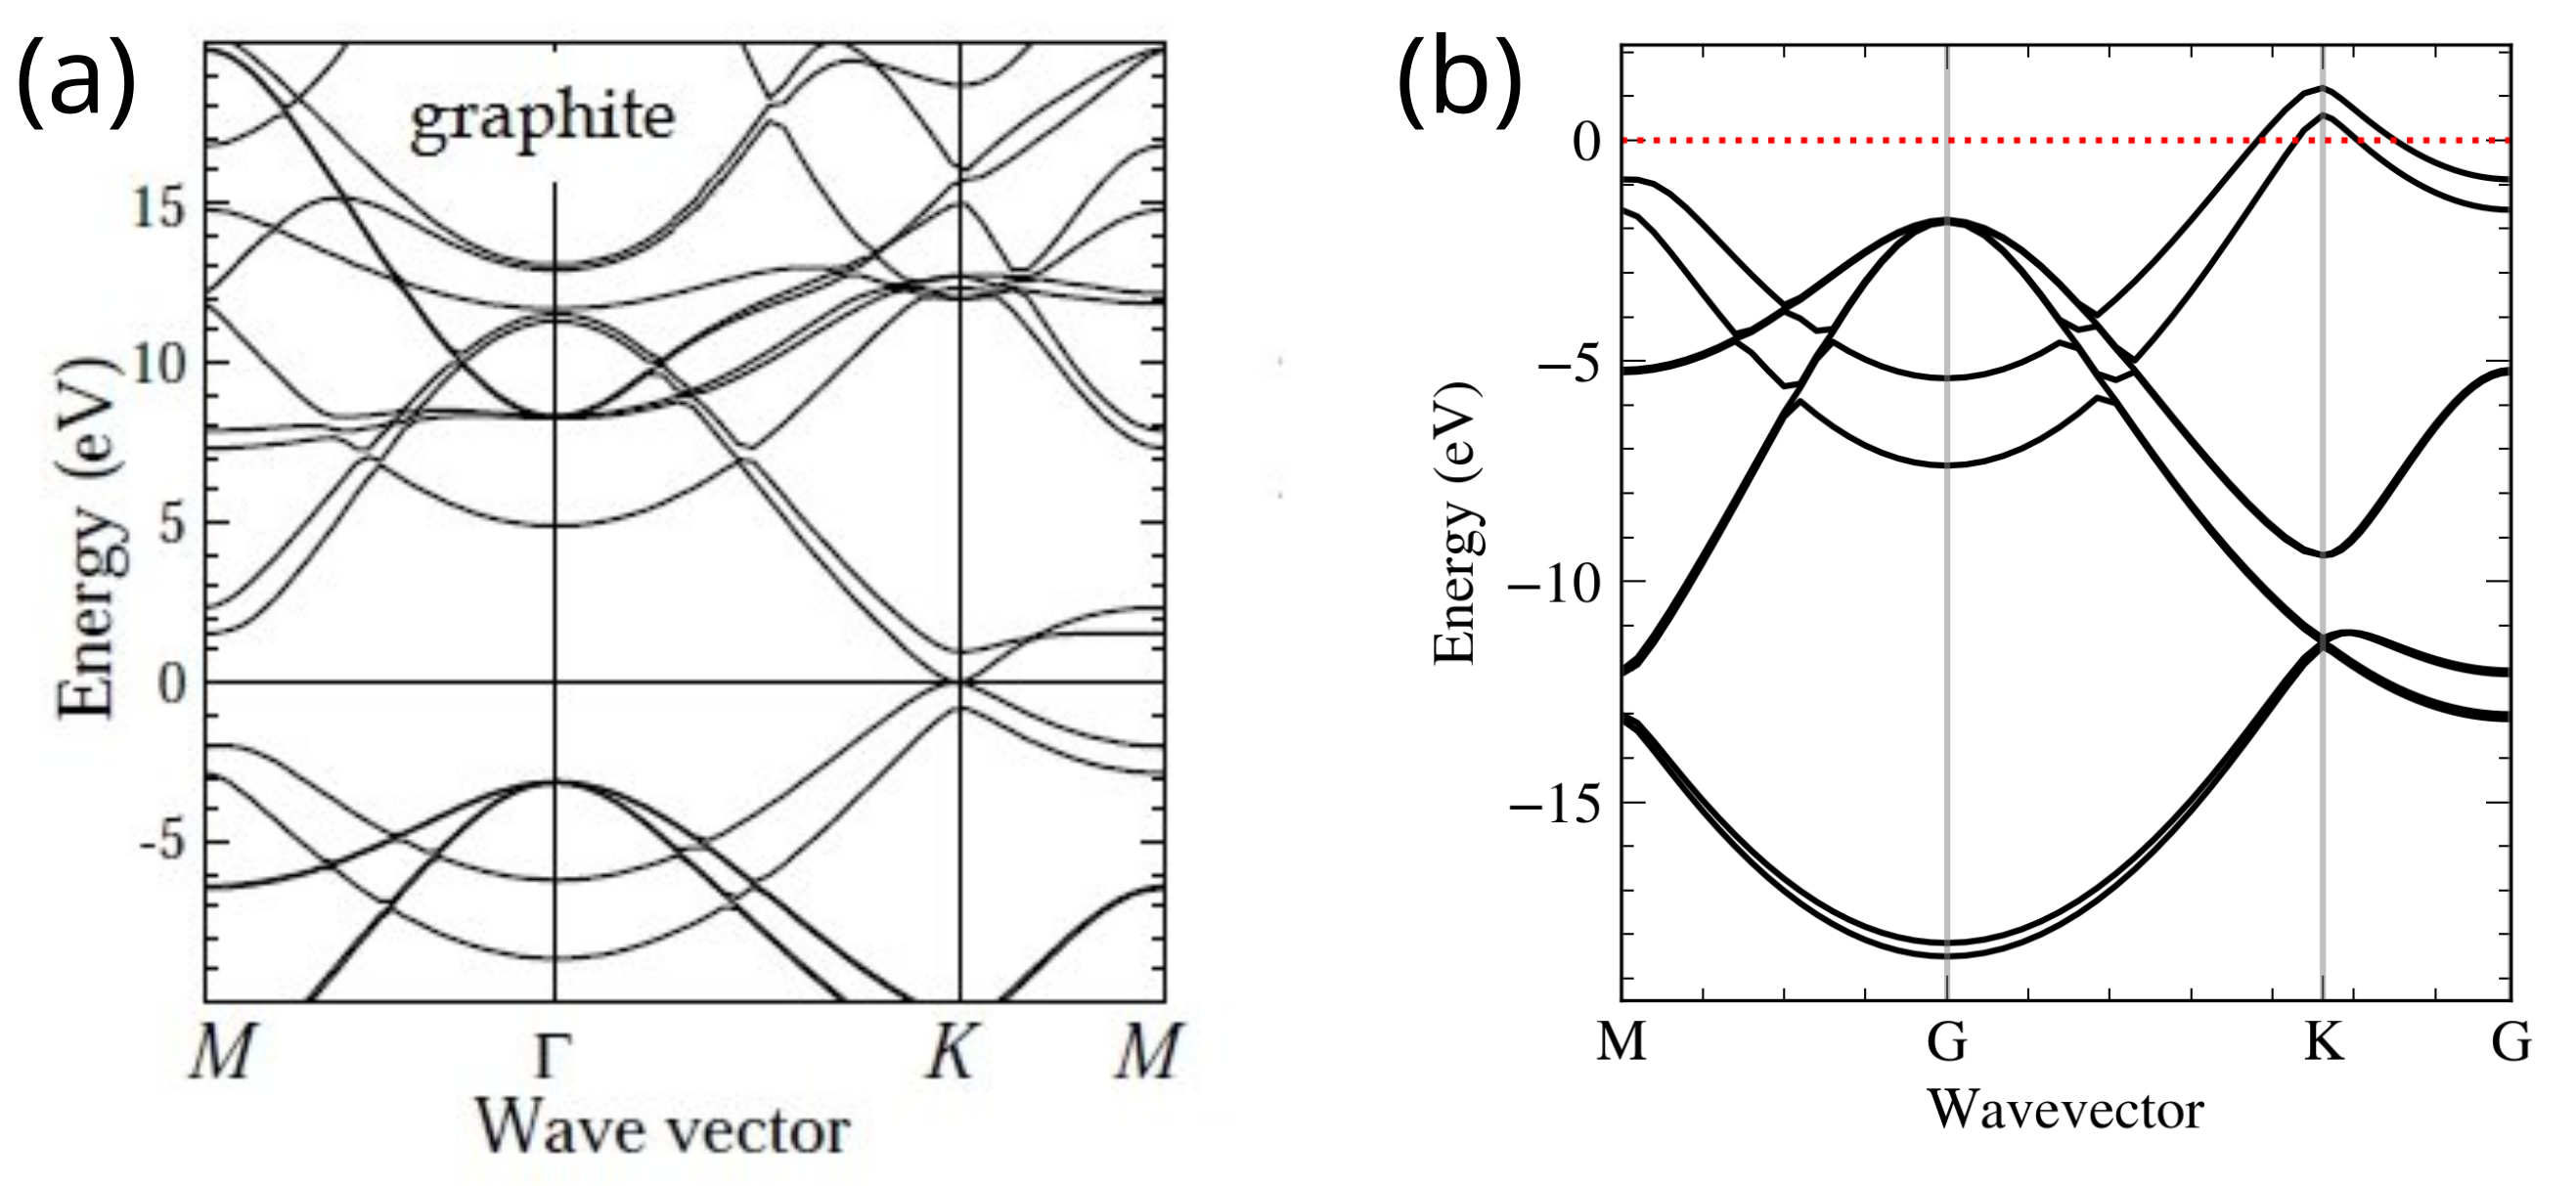
\includegraphics[width = 0.7\textwidth]{figs/ass4_bands_both.png}
    \caption{ The band structure of graphite along the M-G-K-M path for (a) literature \cite{newsonDynamicsCarriersPhotoinjected2010a} and (b) for the optimized structure.}
    \label{fig:ass4_bands}
\end{figure}

\newpage

\printbibliography

% \begin{appendices}
%   \input{Appendix}
% \end{appendices}

\end{document}



